\section{Galaxies-Universe}\linkdest{U}

\subsection{Primordial composition and nucleosynthesis}\linkdest{BBN}

\section{MilkyWay}\linkdest{mw}

\begin{frame}{Refs}
The Gaia-ESO Survey: the Galactic Thick to Thin Disc transition
''The Formation and Evolution of the Milky Way: The distribution of the chemicalelements in our galaxy serves as a "fossil record" of its evolutionary history''
''Stellar Populations and the Formation of theMilky Way'' (Majewski)
\end{frame}

\subsection{Via Lattea e gruppo locale. Teorie di formazione galattica}\linkdest{MWoverview}

\begin{frame}{Milky way: thin/thick disk, halo}
\begin{columns}[T]
\begin{column}{0.5\textwidth}
\begin{figure}[!ht]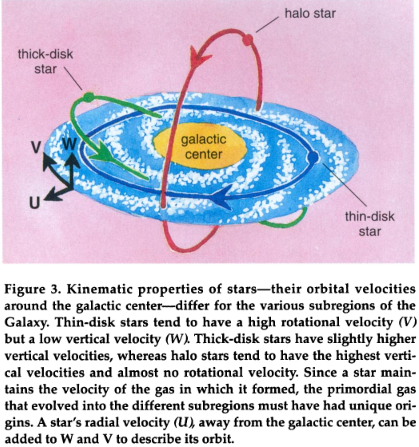
\includegraphics[trim={0cm 0cm 0 0},clip, keepaspectratio,width=0.99\textwidth]{MWcartoon}\label{fig:MWcartoon}\end{figure}
\end{column}
\begin{column}{0.5\textwidth}
\begin{itemize}
\item Thin: $\exv{z}\approx\SI{300}{\parsec}$, Pop I (many metals absorption lines $Z\approx0.013$)
\item Thick: $\exv{z}\approx\SI{1000}{\parsec}$, Pop II (absorption line almost. from H: $Z<0.004$)-Int pop I; kinemat. hot, old, $\alpha$-enh metal poor.
\item Halo: Extreme pop II ($[\alpha/Fe]\approx0.3$)
\end{itemize}
\end{column}
\end{columns}
\end{frame}

\begin{frame}{Milky way: chemical evolution}
\begin{columns}[T]
\begin{column}{0.5\textwidth}
\begin{figure}[!ht]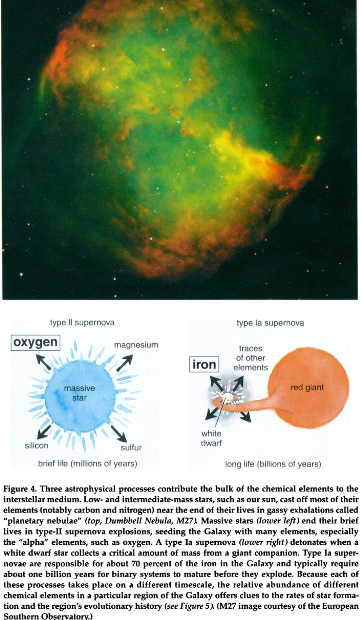
\includegraphics[trim={0cm 0cm 0 0},clip, keepaspectratio,height=0.85\textheight]{PNSNISNII}\label{fig:PNSNISNII}
\end{figure}
\end{column}
\begin{column}{0.5\textwidth}
Massive star: oxigen/$\alpha$-elements (O, Ne, Mg, S, Si, Ca, Ti)
\begin{align*}
&[M/H]=[Fe/H]+\log{(0.694f_{\alpha}+0.306)}\\
&[Fe/H]=\log{(\frac{Z}{X})_*}+1.61
\end{align*}
\end{column}
\end{columns}
\end{frame}

\begin{frame}{Milky way: formation models}
\begin{columns}[T]
\begin{column}{0.4\textwidth}
\begin{figure}[!ht]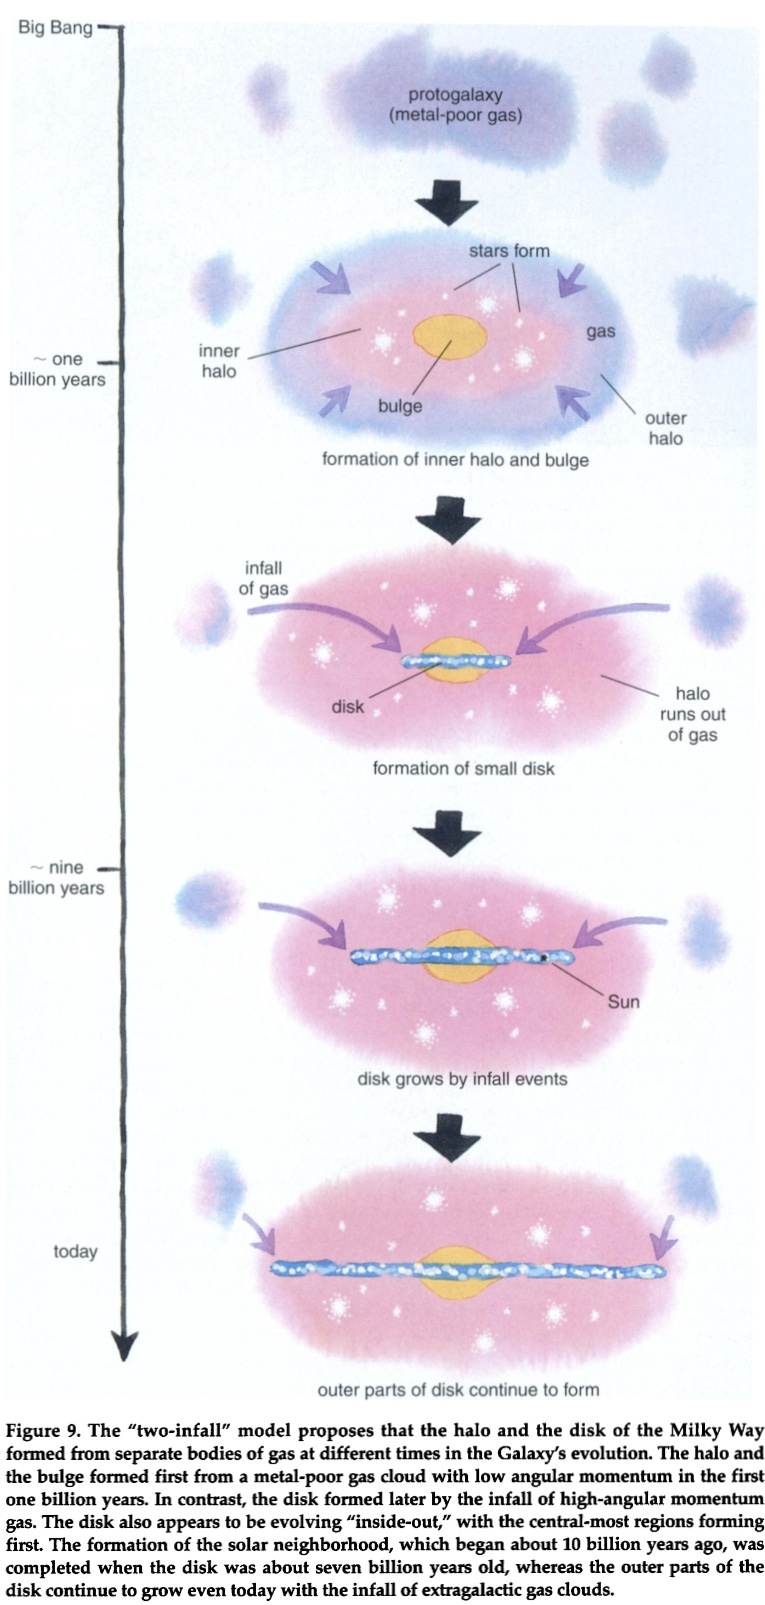
\includegraphics[trim={0cm 0cm 0 0},clip, keepaspectratio,height=0.85\textheight]{MWformation}\label{fig:MWformation}
\end{figure}
\end{column}
\begin{column}{0.6\textwidth}
Two infall model: Low angular momentum materials formed bulge and halo in rapid dissipative collapse (\'a la ELS), mergers with dwarf galaxies (\'a la Searle Zinn) would happened before formation of thin disk: thin disk evolved indipendently from halo from high angular momentum gas, thin disk got thicker in last merger \SI{10}{\giga\year} ago.
Age of thin disk:G dwarf metallicity distribution (Rocha-pinto marciel 1996)
\end{column}
\end{columns}
\end{frame}

\section{Popolazioni stellari}\linkdest{starpop}

\subsection{Problemi osservativi}\linkdest{colormagnitude}

\begin{frame}{Color-Magnitude Diagram}
\begin{columns}[T]
\begin{column}{0.5\textwidth}
\begin{align*}
&M_A=m_A-5\log{d(\si{\parsec})}+5\\
&M_{Bol}=M_{Bol,\odot}-2.5\log{\frac{4\pi R^2F_{Bol}}{\lsun{}}}\\
&=F_{Bol}=\int\,d\lambda F_{\lambda}=\frac{ac}{4}T_e^4\\
&\BC_A=M_{Bol}-M_A
\end{align*}
\end{column}
\begin{column}{0.5\textwidth}
ISM extintion $f_{\lambda}=f_ {\lambda,0}\exp{-\tau_{\lambda}}$, flux at Earth orbit with ISM extintion, $\tau_{\lambda}$ ISM optical depth $\propto\invers{\lambda}$:
\begin{align*}
&m_A=-2.5\log{(\frac{\int_{\lambda_1}^{\lambda_2}f_{\lambda}10\expy{-0.47A_{\lambda}}S_{\lambda}\,d\lambda}{\int_{\lambda_1}^{\lambda_2}f_{\lambda}^0S_{\lambda}\,d\lambda})}-m_0\\
&(A-B)=m_A-m_B
\end{align*}
\end{column}
\end{columns}
\end{frame}

\subsection{Popolazioni semplici}\linkdest{spcpx}

\begin{frame}{SSP: theoretical isochrones}
\begin{columns}[T]
\begin{column}{0.4\textwidth}
\begin{figure}[!ht]
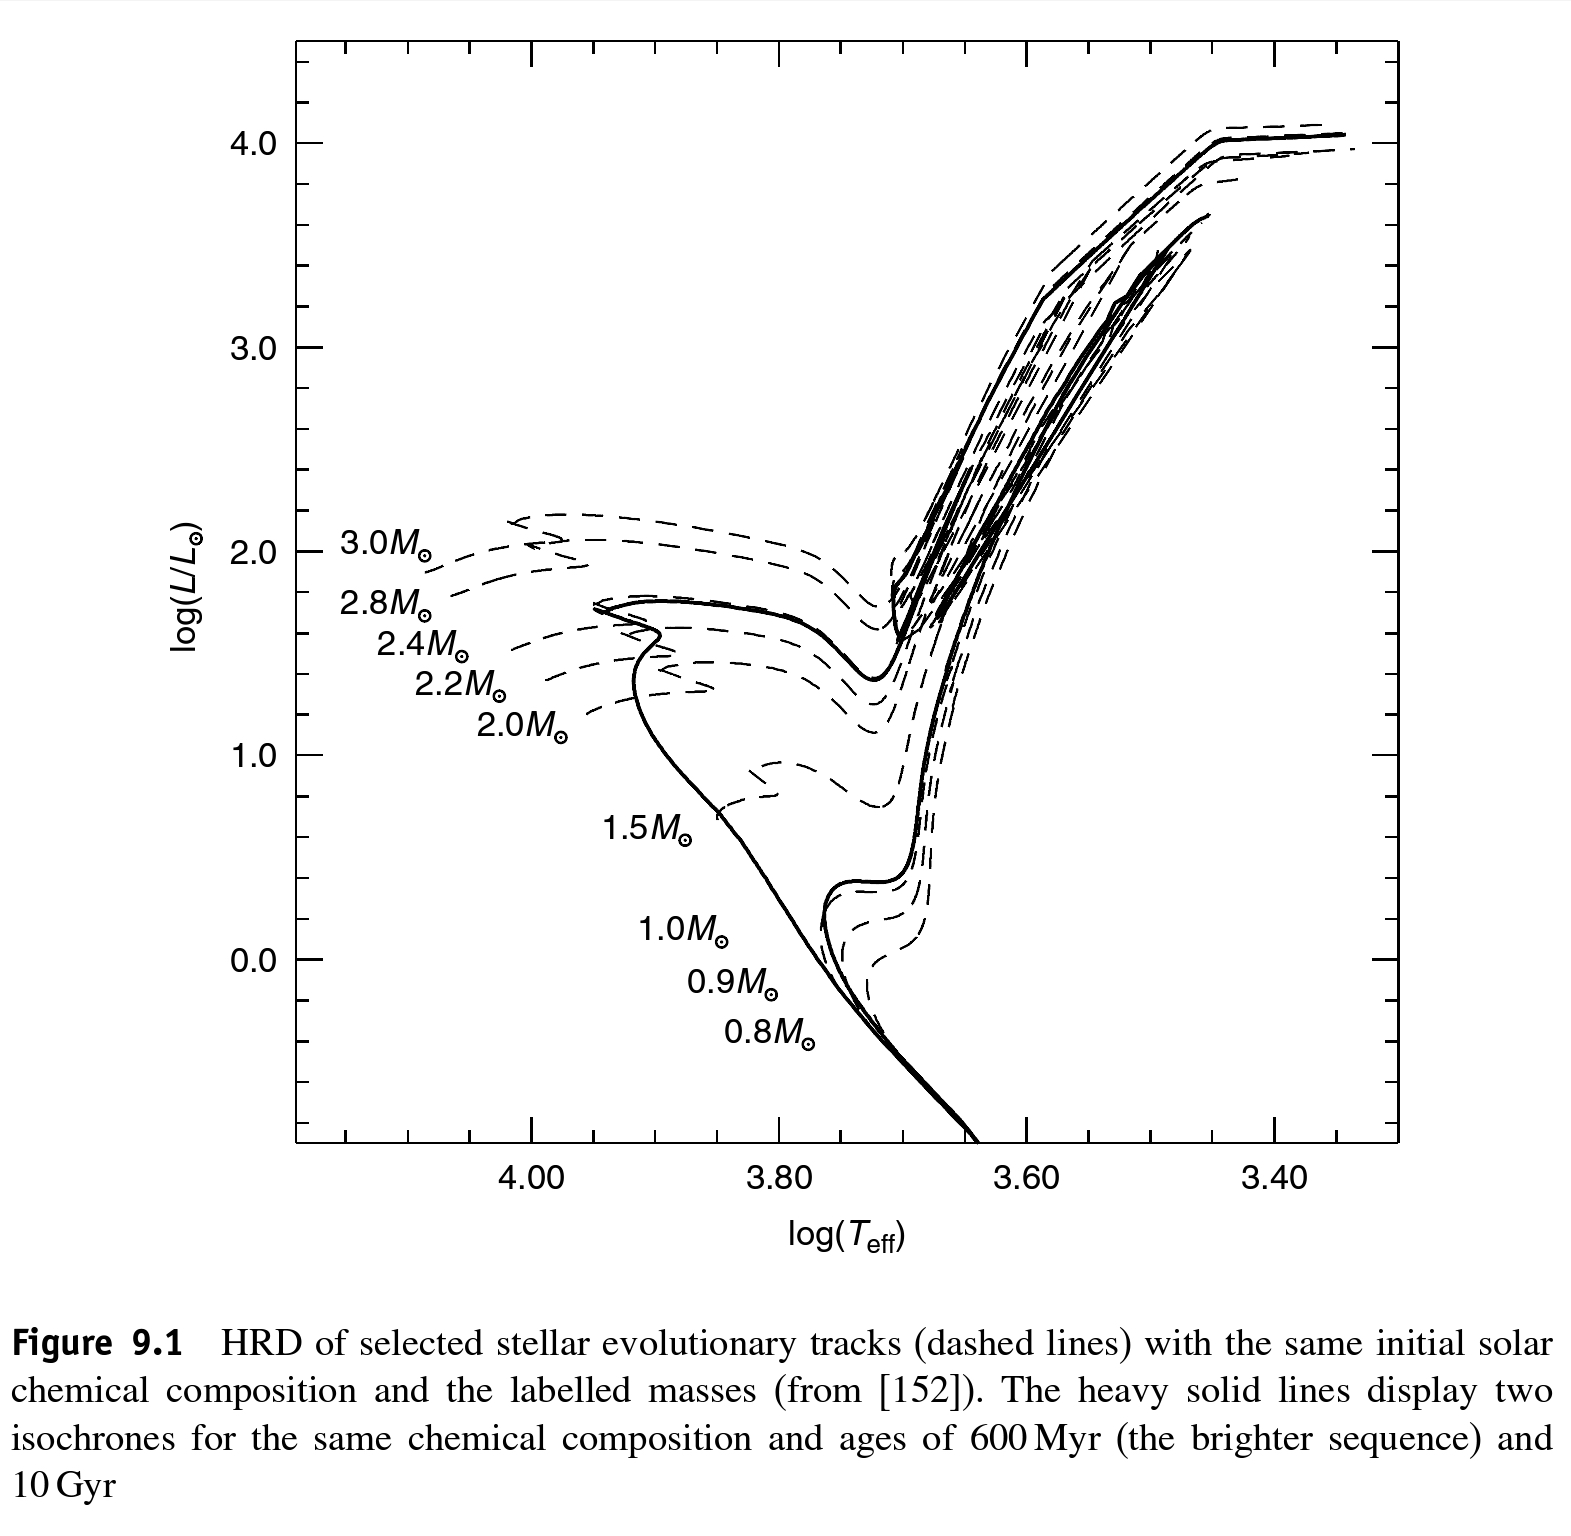
\includegraphics[trim={0cm 0cm 0 0},clip, keepaspectratio,height=0.4\textheight]{isochr}
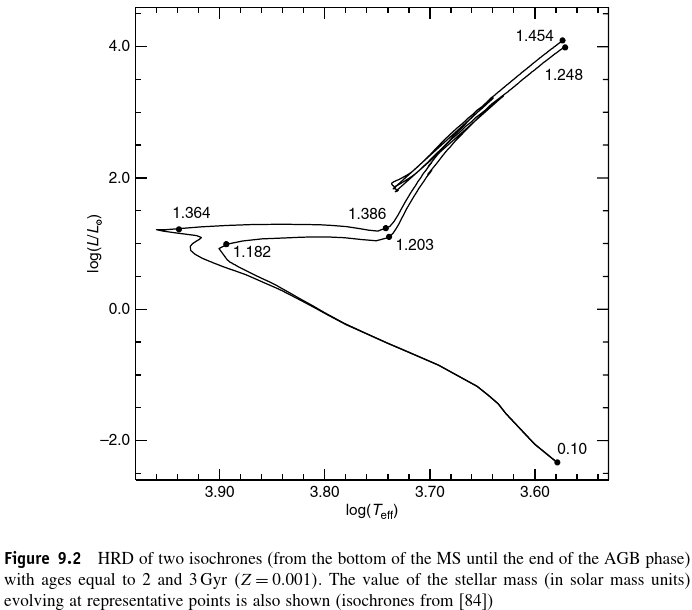
\includegraphics[trim={0cm 0cm 0 0},clip, keepaspectratio,height=0.4\textheight]{SSP-isoMSAGB}
\end{figure}
\end{column}
\begin{column}{0.6\textwidth}
\begin{itemize}
\item Object born at same time in burst of negligible duration with same initial composition; theoretical CMD of SSP is an isochrone at given age.
\item s coordinata lungo isocrona: $\TDy{s}{M}|_t=-\TDy{t}{M}|_s\TDy{s}{t}|_M$ - if rightside close to zero mass evolving in that particular phase is constant
\end{itemize}
\end{column}
\end{columns}
\end{frame}

\begin{frame}{Old SSP: globular cluster and halo star}
\begin{columns}[T]
\begin{column}{0.4\textwidth}
		\begin{figure}[!ht]
		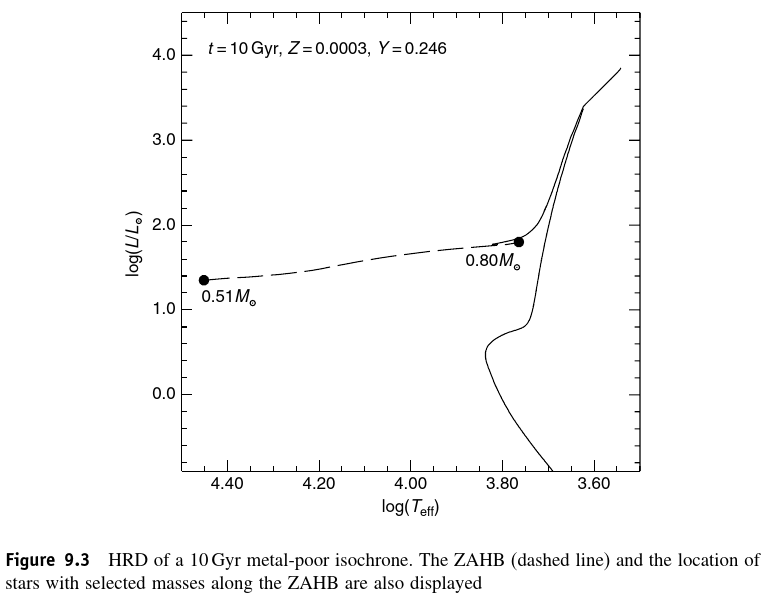
\includegraphics[trim={0cm 0cm 0 0},clip, keepaspectratio,height=0.4\textheight]{SSP-iso10gyrHB}\label{fig:SSP-iso10gyrHB}
		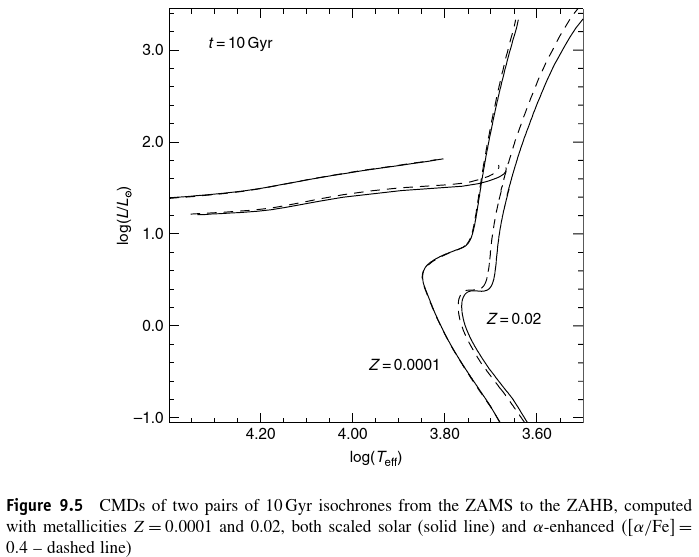
\includegraphics[trim={0cm 0cm 0 0},clip, keepaspectratio,height=0.4\textheight]{SSP-CMDalpha}\label{fig:SSP-CMDalpha}
		\end{figure}
\end{column}
\begin{column}{0.6\textwidth}
		\begin{itemize}
		\item Fig 9.3 shows a \SI{10}{\giga\year} isochrone for metal-poor chem comp typical of globular cluster
		\item $[\alpha/Fe]=0.4$ tipical MW halo - at low Z isochrones are identical - scaled solar are redder and fainter at given Z when traslated to CMD
		\end{itemize}
\end{column}
\end{columns}
\end{frame}

\begin{frame}{Old PPS: globular cluster}
CMD and HRD
\end{frame}

\begin{frame}{Old PPS: open cluster}
CMD and HRD
\end{frame}

\section{Old PSS}\linkdest{oldPPS}

\begin{frame}{Old SSP: effect of ages and Zs}
\begin{columns}[T]
	\begin{column}{0.4\textwidth}
		\begin{figure}[!ht]
		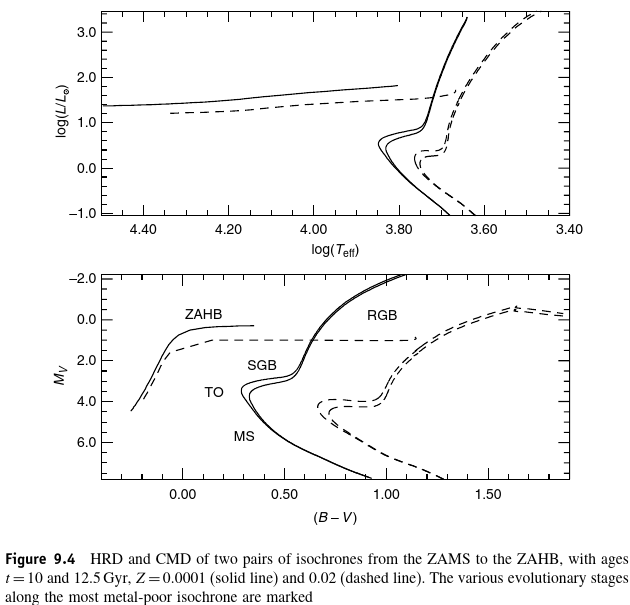
\includegraphics[trim={0cm 0cm 0 0},clip, keepaspectratio,width=0.99\textwidth]{SSP-HDRCMDZpoorMSHB}
		\end{figure}
	\end{column}
	\begin{column}{0.6\textwidth}
		\begin{itemize}
			\item Props of fig 9.4: lower-MS (starting from \SI{2}{\mag} below TO) and RGB unaffected by age but sensitive to Z: lower MS have very long $\tau$ and are still on ZAMS - increasing t-iso lower $M_*$ are at TO hence \xdiminuisce{L_{TO}} - \xaumenta{Z} \xdiminuisce{L_{MS}} compensate the fact that higher Z SSP have higher $M_*$ at TO; RGB depends weakly on $M_*$ and strongly on Z which strongly affect T of RGB; brightness of ZAHB unaffected by age but deps on Z - mostly deps on $M_{cHe}$ at He flash: \xaumenta{Z}, \xdiminuisce{M{cHe}}, age doesn't affect He-core mass for evolving stars RGB stars older than \SI{4}{\giga\year} ($M_*\leq1.2-1.3\msun$);
		\end{itemize}
	\end{column}
\end{columns}
\end{frame}

\begin{frame}{Popolazioni in galassie esterne}
star formation history; popo non risolte semplici e complesse
\end{frame}

\subsection{Indicatori d'et\'a}\linkdest{ageindicator}

\begin{frame}{indicatori di et\'a}
Turn-off/overall contraction: Isocrone di ammassi giovani/vecchi; metodo orizzontale e vertical per ammassi antichi; Lithium depletion boundary per datazione di ammassi giovani
\end{frame}

\begin{frame}{Indicatori di et\'a: metodo verticale}
\begin{columns}[T]
	\begin{column}{0.45\textwidth}
	\begin{figure}[!ht]
	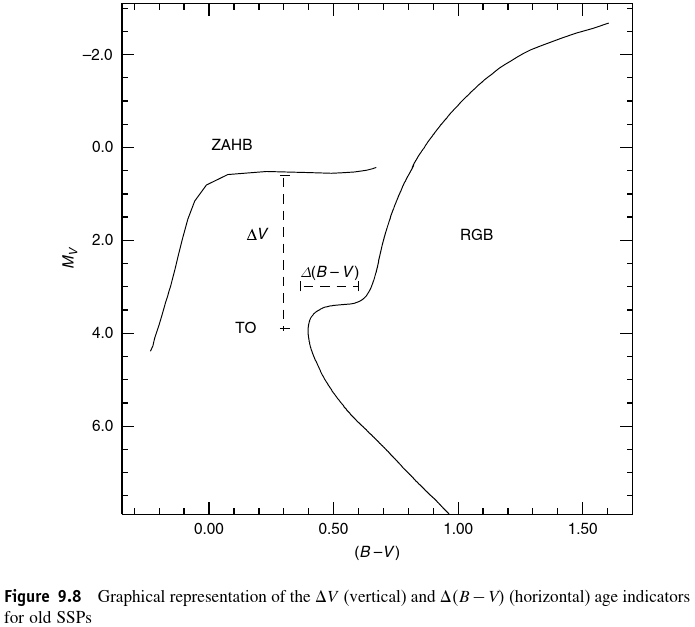
\includegraphics[trim={0cm 0cm 0 0},clip, keepaspectratio,height=0.4\textheight]{SSP-agevert}\label{fig:SSP-agevert}
	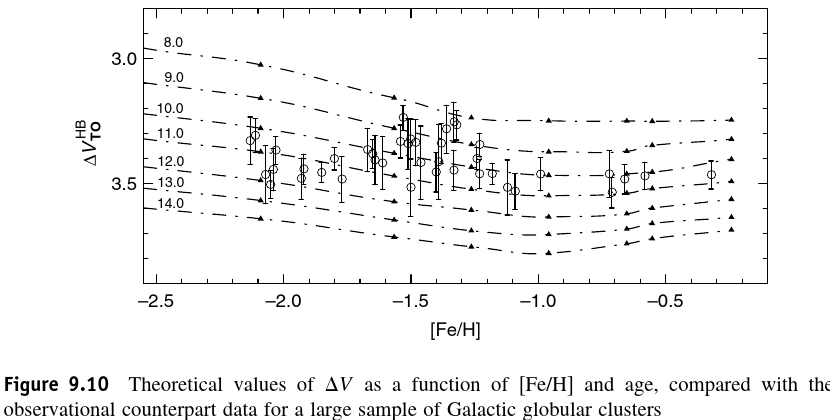
\includegraphics[trim={0cm 0cm 0 0},clip, keepaspectratio,height=0.28\textheight]{SSP-agevertdVZt}\label{fig:SSP-agevertdVZt}
	\end{figure}
	\end{column}
	\begin{column}{0.55\textwidth}
	\begin{itemize}
	\item Comparison between observed and theretical $\Delta V=V_{TO}-V_{ZAHB}$ difference between TO point and ZAHB point at instability strip region around $\log(T_e)\approx3.85$ ($(B-V\approx0.3)$)
	\item ZAHB is unaffected by age: changes of age at given $Fe/H$ changes $\Delta V$ through change in TO-brightness: \xaumenta{t_{age}}, \xaumenta{\Delta V}
	\item At given $[Fe/H]$ a \SI{0.1}{\mag} variation of $\Delta V$ correspond to \SI{1}{\giga\year} in range of oldest star of MW; fixed $\Delta V$ an uncertainty of \SI{0.4}{\dex} in $[Fe/H]$ translate in uncertainty in age about \SI{1}{\giga\year}: at given age TO and ZAHB scale  same way with $[Fe/H]$ - TO region in CMD is vertical so uncertainty about \SI{0.1}{\mag}.
	\end{itemize}
	\end{column}
\end{columns}
\end{frame}

\begin{frame}{Indicatori di et\'a: metodo orizzontale}
\begin{columns}[T]
	\begin{column}{0.45\textwidth}
		\begin{figure}[!ht]
			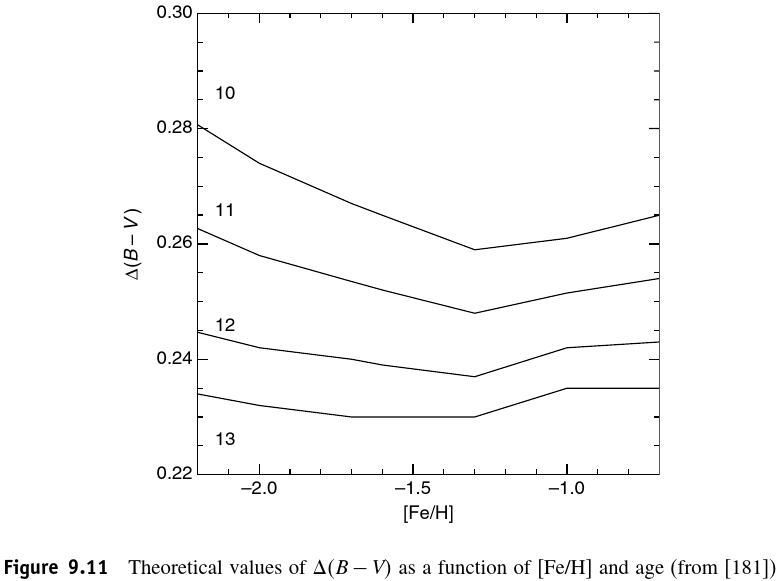
\includegraphics[trim={0cm 0cm 0 0},clip, keepaspectratio,width=0.99\textwidth]{SSP-agehorizdBV}\label{fig:SSP-agehorizdBV}
		\end{figure}
	\end{column}
	\begin{column}{0.55\textwidth}
		\begin{itemize}
			\item $\Delta(B-V)=(B-V)_{RGB}-(B-V)_{TO}$: color difference between TO and base of RGB (color of RGB \SI{2.5}{\mag} above TO) - $(B-V)_{TO}$ varies with t but not $(B-V)_{RGB}$ - not strongly deps on Z since RGB/TO Z-deps cancel out
			\item High accuracy in theretical predictions and observations required: $\frac{\Delta(B-V)}{\Delta t}\approx0.01-0.015\si{\mag\per\giga\year}$ - hardly used for absolute age determination since uncertainties due to color transformation and superadiabatic convection are \SI{0.01}{\mag} but $\Delta(B-V)$ is weakly affected by color trasformation, $Y$ and efficiency of convection around given age
		\end{itemize}
	\end{column}
\end{columns}
\end{frame}

\begin{frame}{Indicatori di et\'a: WD isochrone}
\begin{columns}[T]
	\begin{column}{0.3\textwidth}
		\begin{figure}[!ht]
			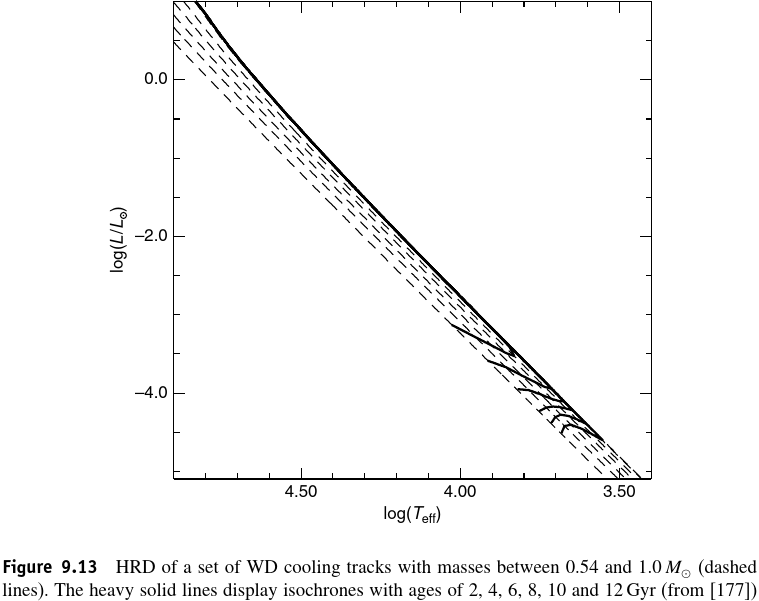
\includegraphics[trim={0cm 0cm 0 0},clip, keepaspectratio,height=0.25\textheight]{SSP-ageWDcool}\label{fig:SSP-ageWDcool}
			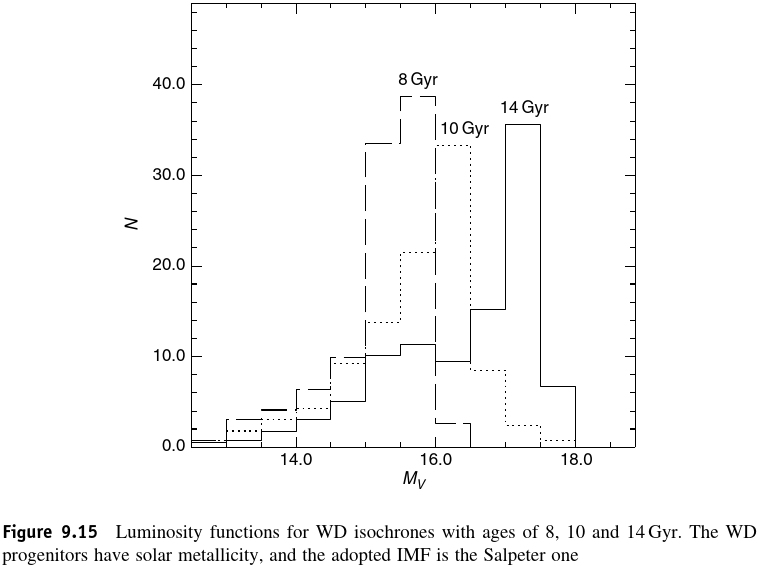
\includegraphics[trim={0cm 0cm 0 0},clip, keepaspectratio,height=0.25\textheight]{SSP-ageWDcoolLF}\label{fig:SSP-ageWDcoolLF}
		\end{figure}
	\end{column}
	\begin{column}{0.7\textwidth}
		\begin{itemize}
		\item we have to extend isochrone to WD stages: brighter part overlaps with cooling track of single WD mass corresponding to WDs produced by stars evolving at end of AGB phase - mass of WD produced by stars evolving along AGB in old population have roughly same mass (the bright part of isochrone), at bottom of isochrone we found object produced by all stars evolved through AGB: higher mass WD produced by higher mass progenitors evolve at smaller radii - left turn at bottom of isochrone
		\item Brightness of bottom end of WD isochrone decreases with age: more advanced cooling stage: can be age indicator if distance is known
		\end{itemize}
	\end{column}
\end{columns}
LF: determined computing progenitor populating WD-isochrone using IMF - Peak of LF and subsequent cut-off corresponds to bottom of isochrone where WD of diff. mass pile-up due to their finite cooling time - increasing age of SSP move peak toward fainter magnitudes - uncertainties due to low luminosity observation and theretical uncertainties on mass loss, EOS of CO-core and envelope, opacity of H/He envelope, boundary conditions.
\end{frame}

\subsection{Indicatori per composizione chimica}

\begin{frame}{Initial Helium abundance}
\begin{columns}[T]
	\begin{column}{0.5\textwidth}
		\begin{figure}[!ht]
			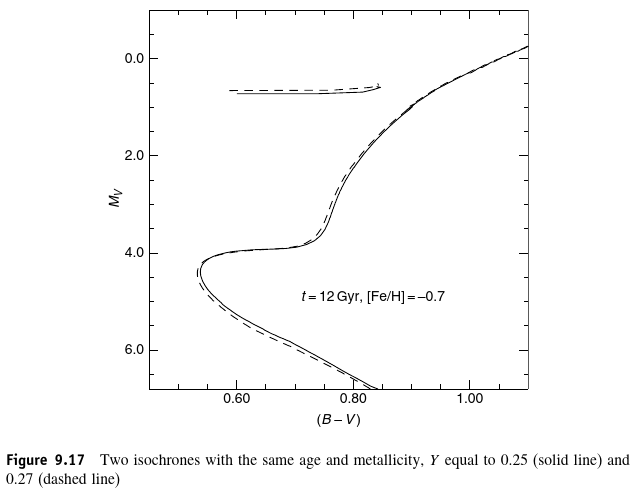
\includegraphics[trim={0cm 0cm 0 0},clip, keepaspectratio,width=0.99\textwidth]{SSP-ageY}\label{fig:SSP-ageY}
		\end{figure}
	\end{column}
	\begin{column}{0.5\textwidth}
		\begin{itemize}
			\item For same age and metallicity mass evolving at TO and post-MS is lower for He-rich isocrones and isochrone shifted to blue from MS to tip RGB - also increases ZAHB brightness and lower TO luminosity at fixed age: \xaumenta{Y}, \xdiminuisce{L_{TO}}, \xaumenta{L{ZAHB}}: \xaumenta{\Delta V} - $\Delta Y\approx 0.02$ causes age decrease \SI{1}{\giga\year}
		\end{itemize}
	\end{column}
\end{columns}
\end{frame}

\begin{frame}{Other Y indicators: parametro $R$ ([44,178]), $\Delta$, $A$}
\begin{columns}[T]
	\begin{column}{0.5\textwidth}
		\begin{figure}[!ht]
			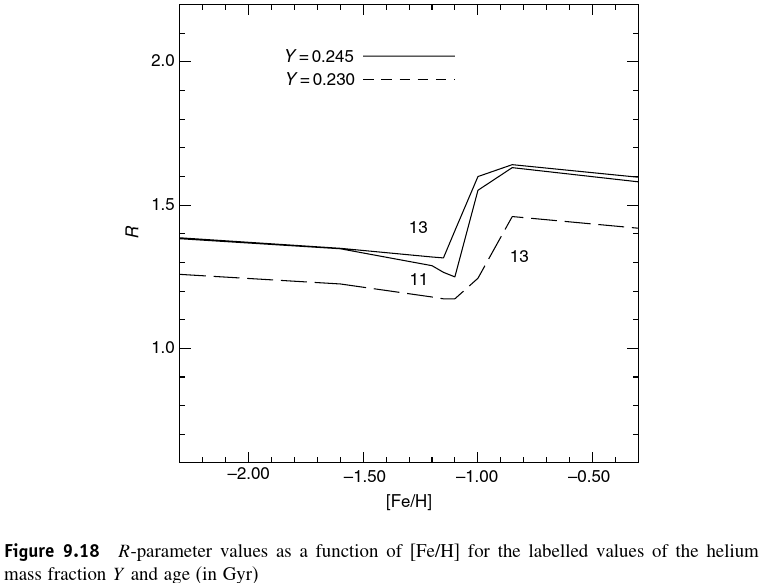
\includegraphics[trim={0cm 0cm 0 0},clip, keepaspectratio,width=0.99\textwidth]{SSP-YRparam}\label{fig:SSP-YRparam}
		\end{figure}
	\end{column}
	\begin{column}{0.5\textwidth}
		\begin{itemize}
			\item Ratio of HB stars to RGB stars brighter than ZAHB: \keyword{R-parameter for Y determination in SSP} $R=\frac{N_{HB}}{N_{RGB}}$
			\item post-MS phases are populated of stars with same initial mass and star count at a stage is proportional to stage evolutionary time - values of masses evolving along RGB and HB and their lifetime are weakly affected by relistic Y variation - \xaumenta{Y}, \xaumenta{L_{HB}}, \xdiminuisce{N_{RGB}}, \xaumenta{R}
			\item Step increase in R when luminosity of RGB bump decreases below ZAHB level due to higher Z
		\end{itemize}
	\end{column}
\end{columns}
\begin{itemize}
\item Parametro $\Delta$: magnitude difference between ZAHB and MS at given colour - at given colour MS becomes fainter and ZAHB brighter when Y increases
\item Mass-Luminosity ratio $A=\log(\frac{L}{\lsun})-0.707\log(\frac{M}{\msun})$: pulsational properties of RR-Lyrae provide Y indicator for old stars - fixed pulsation mode \xaumenta{Y},\xaumenta{L_{HB}},\xaumenta{\exv{M}_{IS}} - $\log(\Pi)=11.627+0.823A-3.506\log(T_e)$
\end{itemize}
\end{frame}

\subsection{Indicatori di distanza}\linkdest{distanceindicator}

\begin{frame}{Distanza ammassi}
main sequence fitting
tip rgb
ZAHB
clump elio
RR lyrae
cefeidi
\end{frame}

\begin{frame}{Parallasse e candele standard ideali. HB fitting}

\begin{align*}
&d=\frac{\SI{1}{\astronomicalunit}}{\tan(p)}\approx\frac{1}{p(\si{\rad})}\si{\astronomicalunit}\\
&d=\frac{\SI{1}{\parsec}}{\tan(p)}\approx\frac{1}{p(\si{\arcsec})}\si{\parsec}
\end{align*}
\keyword{Standard candle}: class of object for which absolute magnitude doesn't change with changing age, Z, etc - determination of distances within our galaxy, Local Group Galaxies and out to Virgo Cluster.
Empirical template: local field stars with known $[Fe/H]$ (spectroscopy) and distance (parallax) and known/negligible reddening ([143, 145]) - limited set of Z.
\keyword{HB-fitting}: observed ZAHB or level of ZAHB at given colour (typically RR-Lyrae IS) is compared to theoretical counterpart - ZAHB brightness is determined by $M_{cHe}$ at He-flash
\end{frame}

\begin{frame}{MS and WD fitting}
\begin{columns}[T]
	\begin{column}{0.5\textwidth}
		\begin{figure}[!ht]
			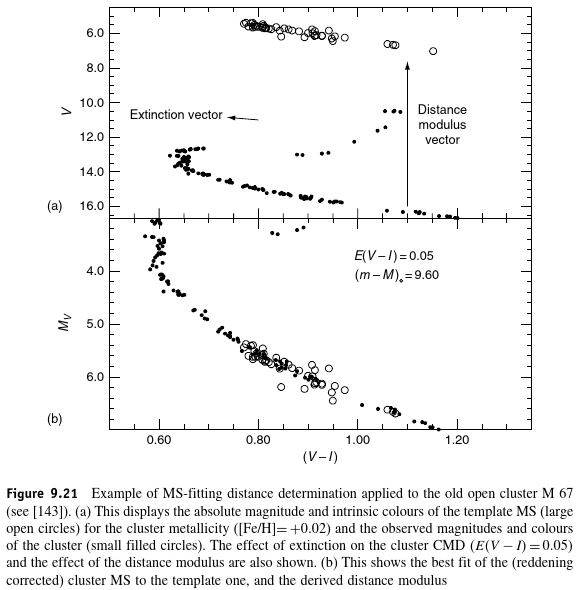
\includegraphics[trim={0cm 0cm 0 0},clip, keepaspectratio,height=0.4\textheight]{SSP-MSfitting}\label{fig:SSP-MSfitting}
			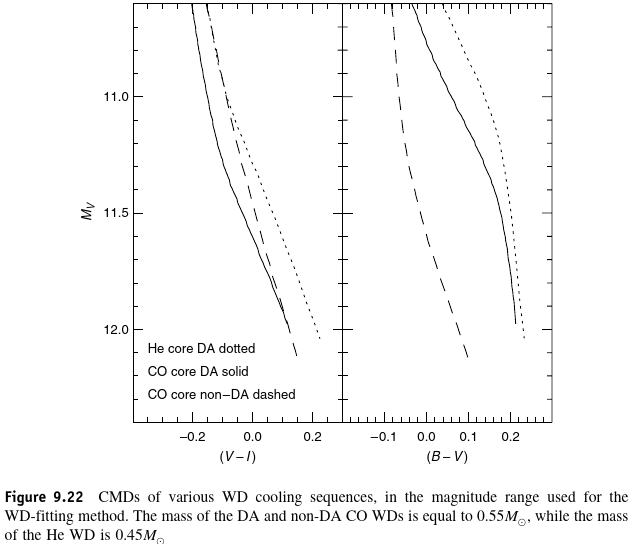
\includegraphics[trim={0cm 0cm 0 0},clip, keepaspectratio,height=0.4\textheight]{SSP-WDfitting}\label{fig:SSP-WDfitting}
		\end{figure}
	\end{column}
	\begin{column}{0.5\textwidth}
		\begin{itemize}
			\item Brightness of lower-MS ($M_V>5.0-5.5$) of old SSP is unaffected by age of stellar pop. - only initial chem comp determine their ZAMS: Y,Z known lower MS can be used as template and compared to observed MS in SSP with same initial chem. comp. - difference between absolute magnitude of template MS and apparent magnitude of observed one provide \keyword{population distance modulus} ($m-M=5\log(\frac{r(\si{\parsec})}{10})$) hence distance in parsec.
			\item Bright part of WD-cooling sequence $M_V\approx10-12$, $T_e=\SIrange{e4}{2e4}{\kelvin}$: stars evolved out of AGB hence $M_*\approx0.55\msun$ - WD are virtually metal free son no color correction needed - but mass have to be known accurately and there is uncertainties on envelope composition
		\end{itemize}
	\end{column}
\end{columns}
\end{frame}

\begin{frame}{Tip of RGB}
\begin{columns}[T]
	\begin{column}{0.5\textwidth}
		\begin{figure}[!ht]
			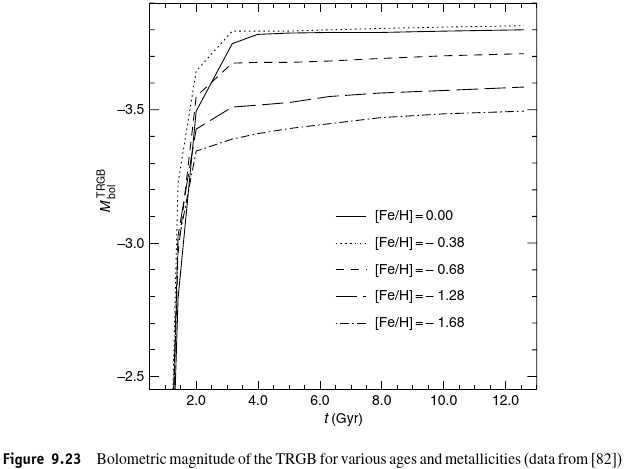
\includegraphics[trim={0cm 0cm 0 0},clip, keepaspectratio,height=0.4\textheight]{SSP-TRGBLtZ}\label{fig:SSP-TRGBLtZ}
			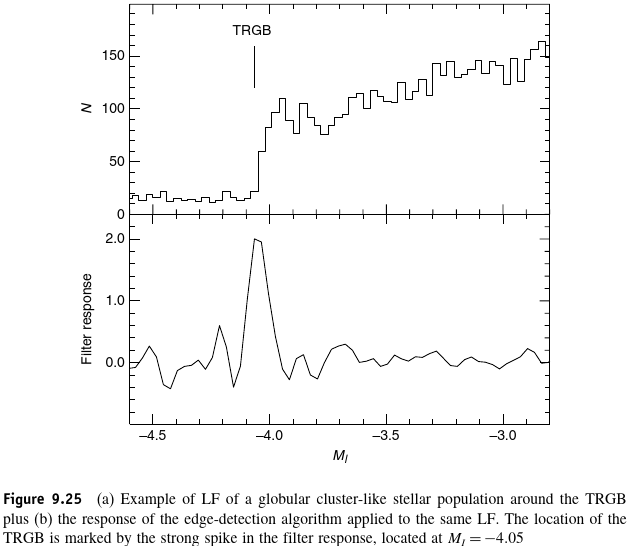
\includegraphics[trim={0cm 0cm 0 0},clip, keepaspectratio,height=0.4\textheight]{SSP-TRGBLFglobar}\label{fig:SSP-TRGBLFglobular}
		\end{figure}
	\end{column}
	\begin{column}{0.5\textwidth}
		\begin{itemize}
			\item Fixed initial composition L of TRGB determined by $M_{cHe}$ at He-flash - lowM stars ignite He with similar core mass (slightly increasing for decreasing initial mass): $M_{bol}^{TRGB}$ is almost constant for $t>\SI{4}{\giga\year}$
			\item At RGB-phase-transition $M_{bol}^{TRGB}$ increses sharply (L decreases) since lifting of \Pelectron-deg in He-core causes He ignition to occur at lower core mass; fixed age $M_{bol}^{TRGB}$ decreases for increasing Z in spite of decreases He-core mass at TRGB
		\end{itemize}
	\end{column}
\end{columns}
\end{frame}

\subsection{Luminosity function And IMF}

\begin{frame}{SSP: luminosity function}
\begin{columns}[T]
	\begin{column}{0.35\textwidth}
		\begin{figure}[!ht]
			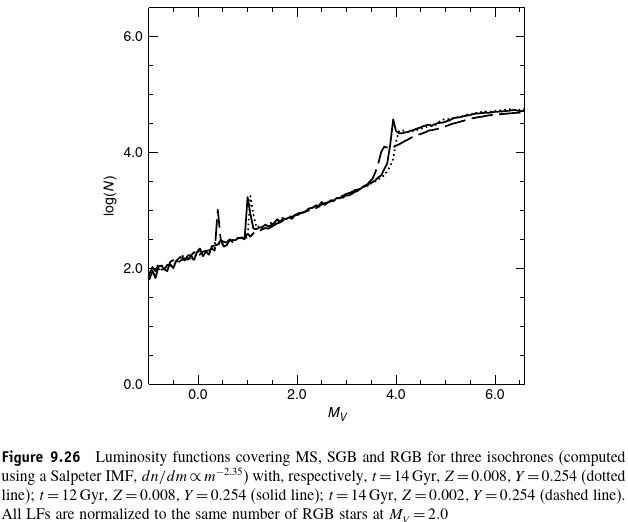
\includegraphics[trim={0cm 0cm 0 0},clip, keepaspectratio,height=0.27\textheight]{SSP-LFMSSGBRGB}
			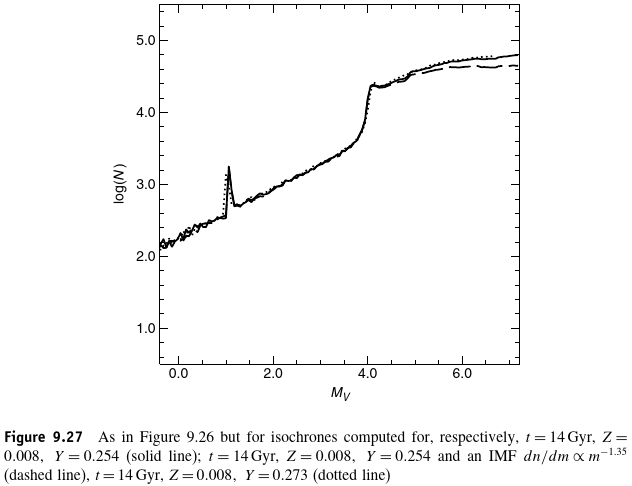
\includegraphics[trim={0cm 0cm 0 0},clip, keepaspectratio,height=0.27\textheight]{SSP-MSSGBRGBsamet}
			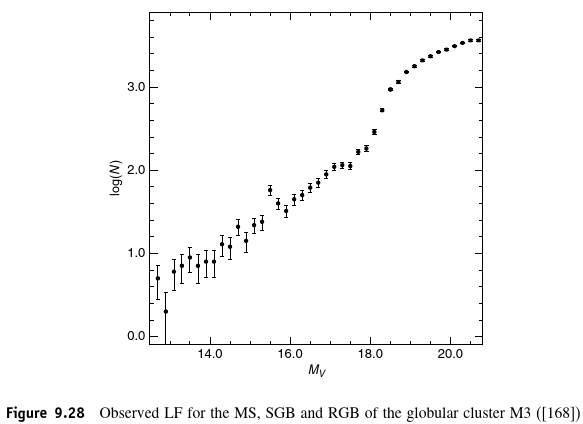
\includegraphics[trim={0cm 0cm 0 0},clip, keepaspectratio,height=0.27\textheight]{SSP-observedLFM3}
		\end{figure}
	\end{column}
	\begin{column}{0.65\textwidth}
		\begin{itemize}
			\item Assess level of agreement stellar evolutionary model/real stars ([43, 56, 159]): contain timescale of stellar evolution, free of uncertainties of surface superadiabatic convection
			\item LF of post-MS fully determined by single mass evolving through that phases - IMF independent; in globular cluster post-MS phases are rel long and well populated
			\item Theoretical LF for old metal-poor SSP as changing Z, age, Y, IMF - normalization at $M_V=2$ at RGB not affected by LF age: MS on r.s., toward brighter $M_V\approx4$ TO, then steep drop of SGB, RGB have more gentle slope - local maximum at RGB bump - whose brightness compared to observations test extension of surface convection $[43]$
			\item Slopes of LFs are quite age-indep. - universality \Pelectron degenerate He-core mass related to L in RGB
			\item MS is sensitive to IMF (populated by large mass range): decreasing Salpeter expo make flatter MS - globular cluster dynamical evolution: \keyword{PFMF}
		\end{itemize}
	\end{column}
\end{columns}
\end{frame}

\section{Young SSP}\linkdest{youngPPS}

\begin{frame}{Young SSP - Age estimate}
\begin{columns}[T]
	\begin{column}{0.4\textwidth}
		\begin{figure}[!ht]
		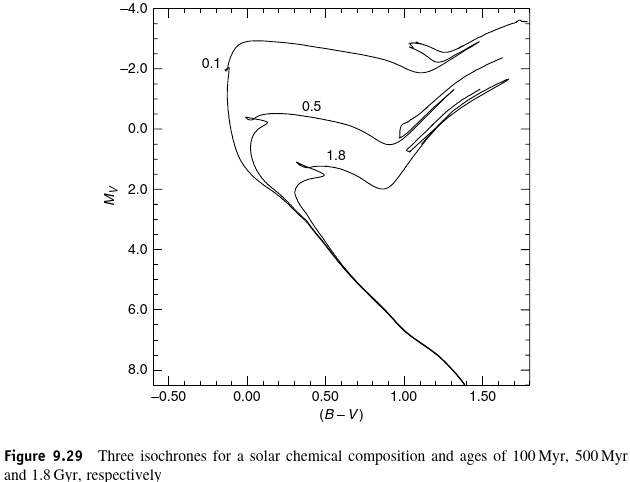
\includegraphics[trim={0cm 0cm 0 0},clip, keepaspectratio,height=0.4\textheight]{SSP-youngisochrones}
		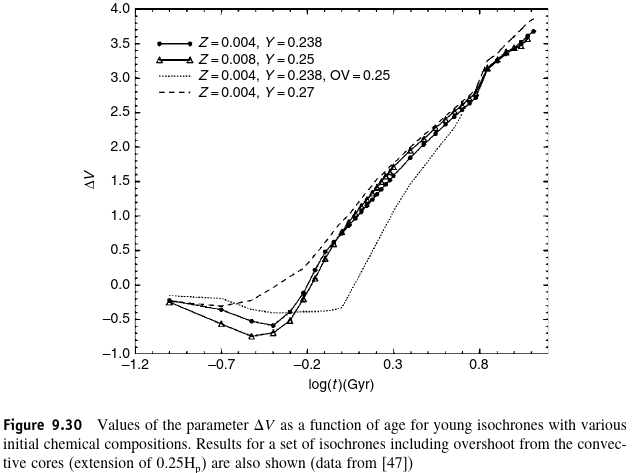
\includegraphics[trim={0cm 0cm 0 0},clip, keepaspectratio,height=0.4\textheight]{SSP-youngagevert}
		\end{figure}
	\end{column}
	\begin{column}{0.6\textwidth}
		\begin{itemize}
		\item Population with $t_{age}<\SI{4}{\giga\year}$ (Galactic open cluster: Praesepe) - isochrone morphology show hook-like feature at TO due to overall contraction - CNO H-burning - and $L_{TO}$ higher - massive stars still evolving in MS - vertical TO region for very young ages
		\item \keyword{TO as age indicator for young SSP} - also He-burning phase is $t_{age}(<2-3\si{\giga\year})$ dependent since He-core along RGB is less degenerate: He-core mass is no longer constant and L at beginning of He-core bunring phase depends on isochrone age.
		\item If distance is known we can fit theoretical isochrones to TO-brightness.
		\item Vertical method using luminosity of He-burning red clump stars
		\item bottom end of WD cooling sequence: for $t_{age}=50-200\si{\mega\year}$ few WD - IMF- and uncertainties of first cooling phase - affected by details of AGB-WD transition/\Pnue-losses
		\end{itemize}
	\end{column}
\end{columns}
\end{frame}

\begin{frame}{young isochrone morphology and population of different evolutionary phases}
\begin{columns}[T]
	\begin{column}{0.5\textwidth}
		\begin{figure}[!ht]
			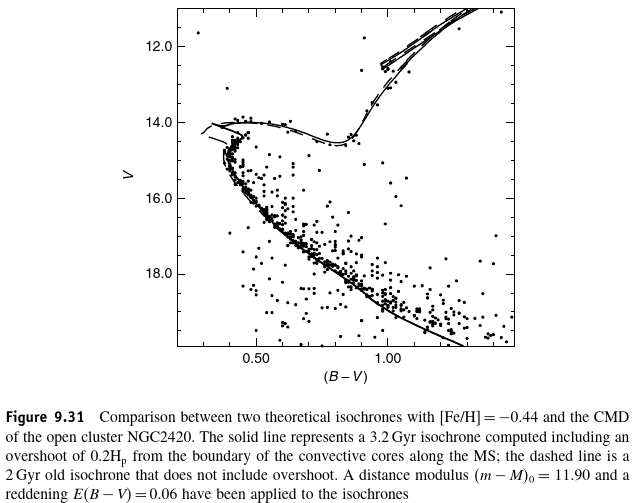
\includegraphics[trim={0cm 0cm 0 0},clip, keepaspectratio,width=0.99\textwidth]{SSP-youngisochOScal}
		\end{figure}
	\end{column}
	\begin{column}{0.5\textwidth}
\begin{itemize}
	\item He-burning phase is red clump close to RGB - RGB is very fast - and $t_{age}<\SI{0.5}{\giga\year}$ He-burning move to blue - longer timescale at blue end of loops
	\item SGB and RGB phases are depopulated (He-core mass reaches $M_{SC}$): can't use horizontal method
	\item \keyword{Overshoot calibration from convective core}: shape of TO region is affected by extension of fully mixed central region - ages fro isochrones including overshoot are higher;
\end{itemize}
	\end{column}
\end{columns}
another possibility is number ratio of MS to He-burning stars $\frac{N_{MS}}{N_{He}}$: due to larger convective core models including core overshoot have larger He-core during He-burning so larger L and lower $\tau_{He}$ while MS lifetime is longer and $\frac{N_{MS}}{N_{He}}$ is larger
\end{frame}

\begin{frame}{Young SSP: Lithium Depletion Boundary}
\begin{columns}[T]
	\begin{column}{0.5\textwidth}
		\begin{figure}[!ht]
			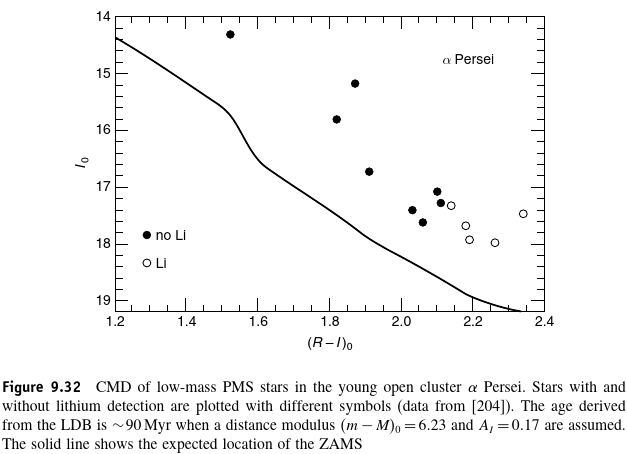
\includegraphics[trim={0cm 0cm 0 0},clip, keepaspectratio,height=0.4\textheight]{SSP-youngLidating}\label{fig:SSP-youngLidating}
			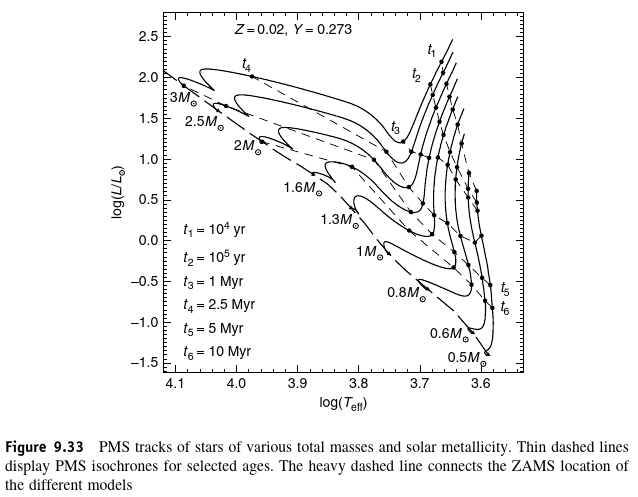
\includegraphics[trim={0cm 0cm 0 0},clip, keepaspectratio,height=0.4\textheight]{SSP-youngPMS}\label{fig:SSP-youngPMS}
		\end{figure}
	\end{column}
	\begin{column}{0.5\textwidth}
		\begin{itemize}
			\item \keyword{LDB} dating method not based on MS/WD models - proton reactions destroy $Li$ where $T>\SI{2.5e6}{\kelvin}$ - $M_*<0.3-0.4\msun$ are fully convective so reaches ZAMS Li-depleted but for $t_{age}<\SI{200}{\mega\year}$ VLM stars are still in PMS and since higher mass star reach $T_{Li}$ earlier one expect to find Li-depleted star above a certain L called LDB - for $t_{age}>\SI{50}{\mega\year}$ VLM stars haven't started Li burning
			\item Comparison of LDB/TO ages contrainsextension of overshoot from convective core of MS star
		\end{itemize}
	\end{column}
\end{columns}
\end{frame}

\begin{frame}{Young SSP: distance indicators}
\begin{itemize}
	\item MS-/WD-fitting
	\item Cepheid $\Pi-L$ relation ($[89]$ for application to LMC): $t_{age}=10-100\si{\mega\year}$ - measuring $\Pi-L$ relationship in two bands allow for determination of distance modulus and extintion
	\begin{align*}
&m_V=M_V+(m-M)_0+A_V\\
&m_I=M_I+(m-M)_0+A_I
	\end{align*}
\end{itemize}
\end{frame}

\section{Popolazioni stellari composite (CSP)}\linkdest{CSP}

\begin{frame}{Complex Stellar Population}
\begin{itemize}
\item \keyword{CSP} are characterized by \keyword{SFH} $\SFH(\SFR,\AMR)$ -  \keyword{star formation rate} (SFR), evolution with time of amount of star formed and their initial chemical composition (Age-Metallicity relation) \keyword{AMR}
\item Time evolution: $M(t)$ total mass, $F(t)/E(t)$ gas accretion/ejection, $e(t)$ stellar mass-loss, $s(t)$ mass in stars, $\Psi(t)$ SFR
\begin{align*}
&M(t)=g(t)+s(t)\\
&\TDy{t}{M}=F(t)-E(t)\\
&\TDy{t}{g}=F(t)-E(t)+e(t)-\Psi(t)\\
&\TDy{t}{s(t)}=\Psi(t)-e(t)\\
&\TDy{t}{(g(t)X_i(t))}=e_{X_i}(t)-X_i(t)\Psi(t)+X_i^F(t)F(t)-X_i(t)E(t)
\end{align*}
\end{itemize}
Above equations coupled stellar evolution models could reproduce chemical and spectrophotometric evolution of CSP.

Determination of SFR and AMR from observed CMD: simulate observed CMD of CSP as linear combo of CMD of elementary population with homogeneous age and metallicity distribution within small age and Z range centered around discretized value of t/Z.
\end{frame}

\begin{frame}{Determination of SFH of CSP}
\begin{itemize}
\item Si divide CMD in celle in maniera da avere abbastanza stelle per ogni cella e abbastanza celle per ogni fase evolutiva, $N_o(i)$ numero di stelle nella cella i
\item Si generano CMD sintetici di popolazioni stellari elementari j con distribuzione di et\'a e metallicit\'a uniforme in $\Delta t$ e $\Delta z$ centrati attorno a n valori t,m (AMR and SFR constant within $\Delta t$ e $\Delta z$ bin): using MC technique to draw mass according to IMF and uniform distro in age and metallicity we determine CMD interpolating within grid of isochrones; another free parameter can be fraction of unresolved binary; account for foreground contamination - $N_s(i)=\sum_ja_jN_e^j(i)$ compared with observed with $\chi^2=\sum_i\frac{(N_o(i)-N_s(i))^2}{N_o(i)}$, the $1\sigma$ confidence interval on each parameter is defined by $\Delta\chi^2=\chi^2-\chi^2_{min}$; in presence of Poisson errors $[65]$ as equivalent to $\chi^2$ can be $-2\ln{(PLR)}=2\sum_iN_s(i)-N_o(i)+N_o(i)\ln{\frac{N_o(i)}{N_s(i)}}$
\end{itemize}
\end{frame}

\begin{frame}{Distance indicators: TRGB}
Resolved CSP CMD can be used to estimate distances for cosmological distance calibration, study of local deviation from hubble flow, relative distance analysis for group of galaxies, comparison of intrinsic properties of some classis of stars in diff environments.
\keyword{TRGB as degenerate distance indicator for CSP}: TRGB if bright part of RGB is detected: an SFH like LMC (or SMC) produces a CMD with an RGB similar to RGB of galactic globular cluster however LMC's RGB have mean age of \SI{4}{\giga\year} - in low mass star ratio between RGB and MS timescale increases for increasing stellar mass until $M_*\approx1.6\msun$: in case of constant SFR stat-weight of RGB sample related to younger population is therefore larger than that of older RGB stars; if $Z\gtrsim-0.7$ Z-dep of $M_I^{TRGB}$ is high and wrong Z causes wrong distance (ie \SI{4}{\giga\year} old RGB are bluer than that \SI{12}{\giga\year} old); if real age gets closer to \SI{2}{\giga\year} the TRGB luminosity declines as deg-nondeg He core transition approaches thus inducing error when globular cluster calibration is used
\end{frame}

\begin{frame}{Distance indicators: RR-Lyra, Cepheids and HB}
\begin{itemize}
\item RR-Lyra can be used averaging their apparent magnitude to estimate CSP distance by applying the HB absolute magnitude calibration: HB level is strongly affected by metallicity
\item CSP can be populated by HB object with mixture of Z and ages: also age can affect HB level for less then few \si{\giga\year} - the only way to extimate absolute magnitude of He-burning stars is to build synthetic CMD with population SFH: diff between mean V magnitude of He burning in solar neighborhood and in LMC as predicted by SFH estimate is $0.26$ mag, for globular cluster like age magnitude difference cinsidering only diff. of mean $Z$ of two HB pop is $\approx0.1$ mag in V
\item Cepheid are the most used to determine distance from CSP harbouring young stars: also P-L relation can be Z dep: given narrow age covered by C one doesn't expect substantial chem evol.
\end{itemize}
\end{frame}

\begin{frame}{Planetary Nebula LF}
\begin{itemize}
\item PN are bright objects with L greater than $L_{TRGB}$; used for distance indicator in low/int-$M_*$ ($t>\SI{e8}{\year}$)
\item $[109]$: observations show that number of PN as function of $F_{5007}$ $OIII$ emission line is constant among galaxies of various type - constant value of absolute cut-off $M_{c}=\num{-4.48+-0.036}$
\begin{align*}
&m_{5007}=-2.5\log{F_{5007}}-13.74\\
&N(m_{5007})=\exp{0.307m_{5007}}[1-\exp{3(m_{cf}-m_{5007})}]
\end{align*}
\end{itemize}
\end{frame}

\section{Unresolved stellar population}\linkdest{USP}

\begin{frame}{Stellar population in distant galaxies}
\begin{itemize}
\item In distant galaxies we can't resolve stars: photometry and spectroscopy can provide integrated magnitudes, colours and spectra of the population
\item CSP: estimate mean age and metallicity comparing integrated colour or line indices with calibrations for SSP
\end{itemize}
\begin{figure}[!ht]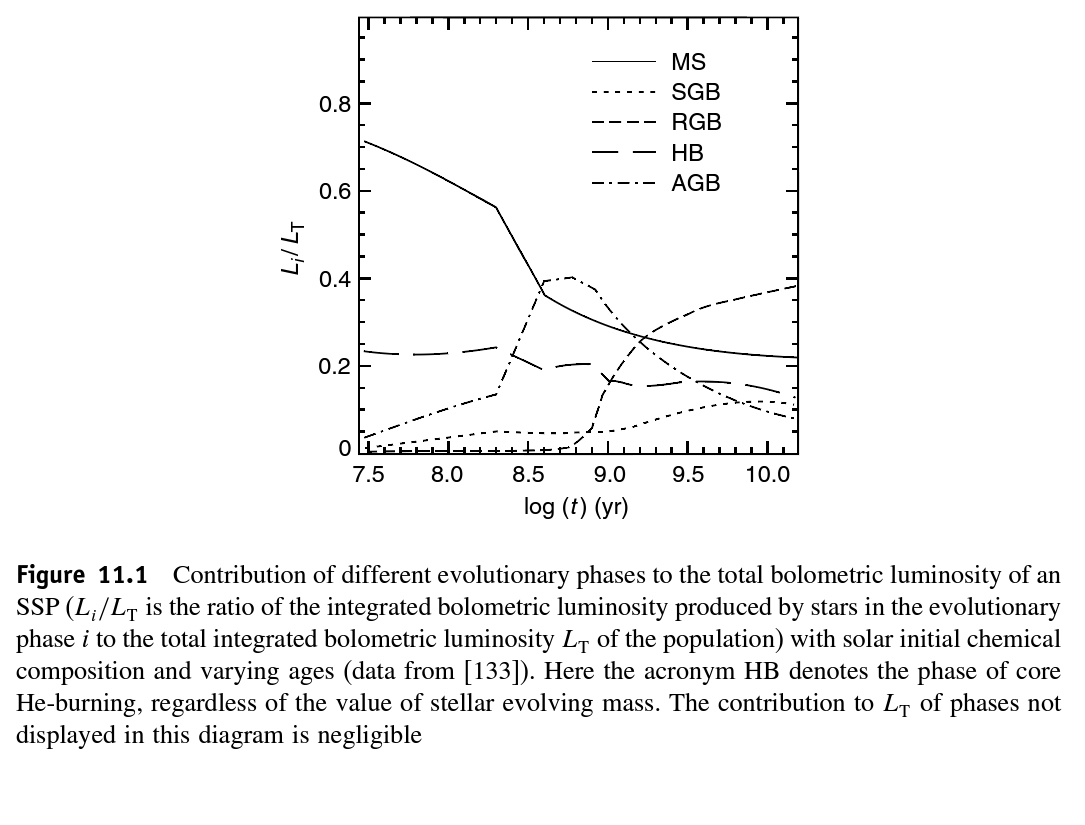
\includegraphics[trim={0cm 0cm 0 0},clip, keepaspectratio,width=0.45\textwidth]{Lphasesunresolved}~
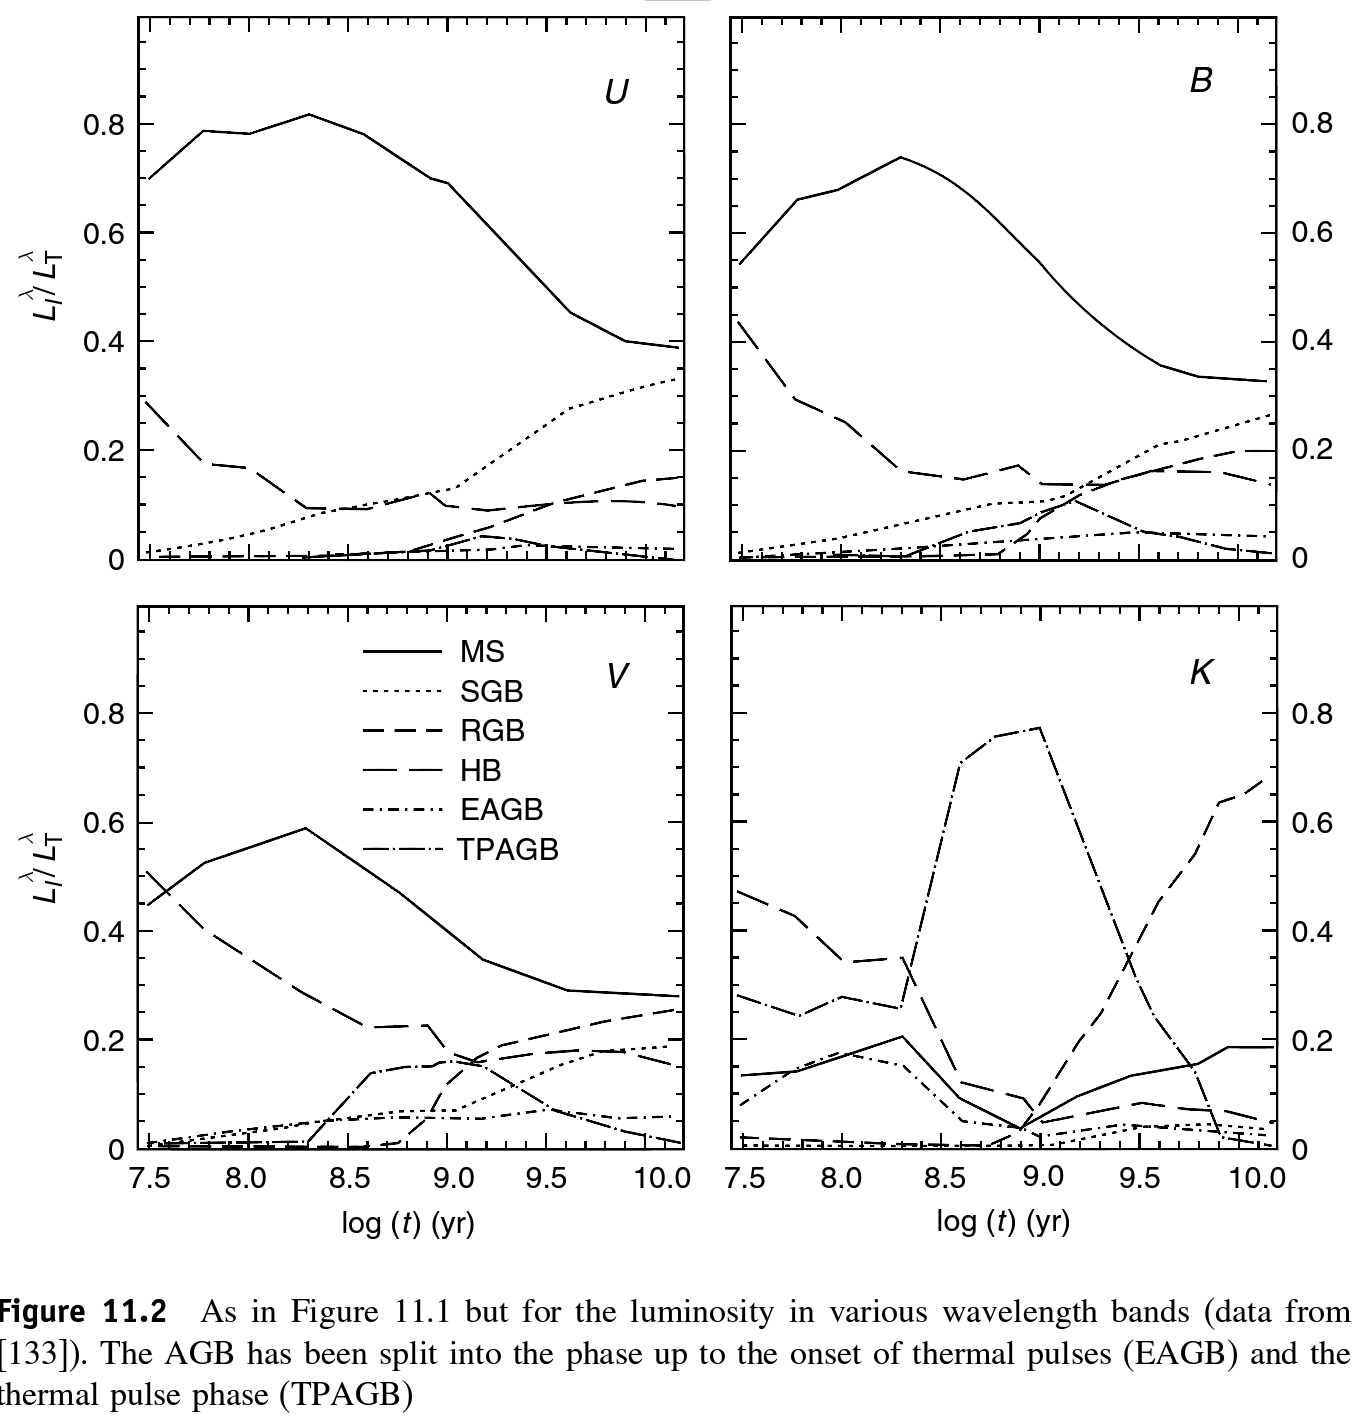
\includegraphics[trim={0cm 0cm 0 0},clip, keepaspectratio,width=0.45\textwidth]{unresolvedbandphases}
\end{figure}
\end{frame}

\begin{frame}{Unresolved SSP}
Monochromatic integrated flux: $F_{\lambda}^I(t,Z)=\int_{M_l}^{M_u}f_{\lambda}(M,t,Z)\phi(M)\,dM$, $M_u$ initial mass of star evolving through WD at SSP age approx $M_{TO}$, contribute to integrated flux of WD is negligible - for $T<\SI{300}{\mega\year}$ MS is largest contributor to $L_T$, for $\SI{300}{\mega\year}<t<\SI{2}{\giga\year}$ AGB is largest contri due to evolving mass original between $7-2\msun$ that have large luminosity due to massive CO-core; $t>\SI{2-3}{\giga\year}$ RGB takes becomes major contributor to $L_T$ that now harbours low-mass long life/brighter stars

\end{frame}